% !TeX encoding = UTF-8
% !TeX spellcheck = en_US

\documentclass[
	paper=A4,
	parskip=full,
	chapterprefix=true,
	11pt,
	headings=normal,
	bibliography=totoc,
	listof=totoc,
	titlepage=on,
]{scrreprt}

\usepackage{../../lieb}

\usepackage{feynmp}
\DeclareGraphicsRule{.1}{mps}{*}{}

\graphicspath {{../images}}

\heads{RWTH Aachen \\ Particlephyics Lab}{T17 \\ W-Boson}{Lieb | Stettner \\ \today} 
\date{\today}

\newcommand{\MET}{\ensuremath{{\slashed{E}_\mathrm{T}}}\xspace}
\newcommand{\ELET}{\ensuremath{{E_\mathrm{T}^\mathrm{el}}}\xspace}

\newcommand{\thirdwidth}{0.32\textwidth}
\newcommand{\halfwidth}{0.48\textwidth}
\newcommand{\fullwidth}{1.0\textwidth}

\setlength\parindent{0pt}
\setlength{\parskip}\medskipamount

\title{Particle Physics Laboratory Class \\ \quad \\ Experiment T17 | W-Boson }
\author{Jonas Lieb, (312136) \\ Jöran Stettner (312169) \\ \\  RWTH Aachen}

\newcommand{\dnull}{D$\slashed{\mathrm{0}}$\xspace}

\begin{document}

\maketitle

\cleardoublepage

\setcounter{tocdepth}{2}
\tableofcontents

\cleardoublepage

\chapter{Introduction}

This analysis deals with \PW-Boson physics conducted at the \dnull experiment at the Tevatron accelerator (FERMILAB, Chicago). The data has been taken in proton-antiproton collisions at a center-of-mass energy of $\sqrt{s} = \SI{1960}{\giga\electronvolt}$.

\section{Units}
In this report, a natural unit system of particle physics is used: first, the speed of light and Planck's constant are fixed:
\begin{equation}
c \defeq \num{1},\quad \hbar \defeq \num{1}
\end{equation}
From this convention, many quantities arise in units of energy. Additionally, the gigaelectronvolt (\si{\giga\electronvolt}) is chosen as basic energy unit, in order to deal with numbers of magnitude $\order{1}$.

\subsection{\PW-Boson Production and Decay}
The process of interest is the \PW-Boson production from the valence quarks of the protons and antiprotons, and the decay into an electron and an electron neutrino.
\begin{equation}
	\Pproton\APproton \rightarrow \PWminus \rightarrow \Pelectron \APnue
\end{equation}
Equivalently, there exists a oppositely charged process:
\begin{equation}
\Pproton\APproton \rightarrow \PWplus \rightarrow \Ppositron \Pnue
\end{equation}
With the assumption that the \PWplus and \PWminus have similar properties (except the electric charge), one does not expect any difference between the processes. Because of that, the analysis will not differentiate between them and treat positrons as electrons in the final state.

Both processes combined have an expected cross section\cite{HBK+2013Experiment} of 
\begin{equation}
	\sigma = \SI{2.58 +- 0.09}{\nano\barn}
\end{equation}
and should show a resonance at the predicted \PW-Boson mass\cite{Oo2014Review} of 
\begin{equation}
	m_{\PW} = \SI{80.385 +- 0.015}{\giga\electronvolt}
\end{equation}

\section{The \dnull Detector}
The measurement took place in 2004 until 2006 at the \dnull experiment at FERMILAB. The \dnull detector is a cylindrical particle detector located around the Tevatron beam pipe. It consist of a silicon tracker in the center region, enclosed by an Argon electromagnetic calorimeter.

Inside the detector, a Cartesian coordinate system and a cylindrical coordinate system are used. The origin of both systems lies in the interaction point, with the z-axis pointing along the beam pipe. The angle $\phi$ is measured in a plane perpendicular to the z-axis. 

Because the colliding protons are composite particles, the longitudinal momentum of the interacting quarks is unknown. The transversal components, however, are zero in the initial state. From momentum conservation it follows that the sum of all transversal momenta in the final state is also zero. 
To represent this conservation in the transversal plane, energies and momenta are projected onto it. This introduces the transverse electron energy \ELET.
Another important definition is the missing transverse energy \MET. 


\chapter{Monte-Carlo Samples}



\chapter{Selection of Events}
In this chapter, the measured variables are introduced and the selection of events is explained. \\
The distributions of the measured and simulated quanities are shown in figures \ref{no_cuts_Ets}, \ref{nocuts_etaphi} and \ref{nocuts_dziso}. It becomes clear that the MC did not simulate all processes which occur in the detector, see for example the double-bump structure in the distribution of transverse electron energy. To perform the analysis as sketched above, it is important to select only those events which fall in regions where data and MC are in good agreement. Otherwise, a discrepancy coming from background processes would be interpretated as a mismatch to the simulated W-mass. Among others, these background processes are possible: 
\begin{itemize}
	\item $\Ppizero \rightarrow 2 \Pphoton$ decays which could account for the lower electron energies.
	\item Jets which are misidentified as electrons. The electron isolation variable becomes smaller in this case.
	\item $\PZ \rightarrow \Ppositron \Pelectron$ decays where one of the leptons leaves the detector unnoticed.
\end{itemize}

To constrain the analysis to regions of good agreement between MC and data, the following cuts are applied to all events:
\begin{table}[htbp]
	\centering
	\begin{tabular}{ 
			l 
			l
			l
			l
		}
		\toprule
		{Quantity} & {Threshold} & { } \\ 
		\midrule
		\MET & $>\SI{20}{\giga\electronvolt}$ & \\
		\ELET & $>\SI{30}{\giga\electronvolt}$ & No low energy electrons (e.g. \Ppizero) \\
		
		\bottomrule
	\end{tabular}
	\caption{Ergebnisse von Anpassungen für verschiedene Bereiche}
	\label{tbl:diode}
\end{table}


\begin{figure}%
	\centering
	\begin{subfigure}{0.45\textwidth}
		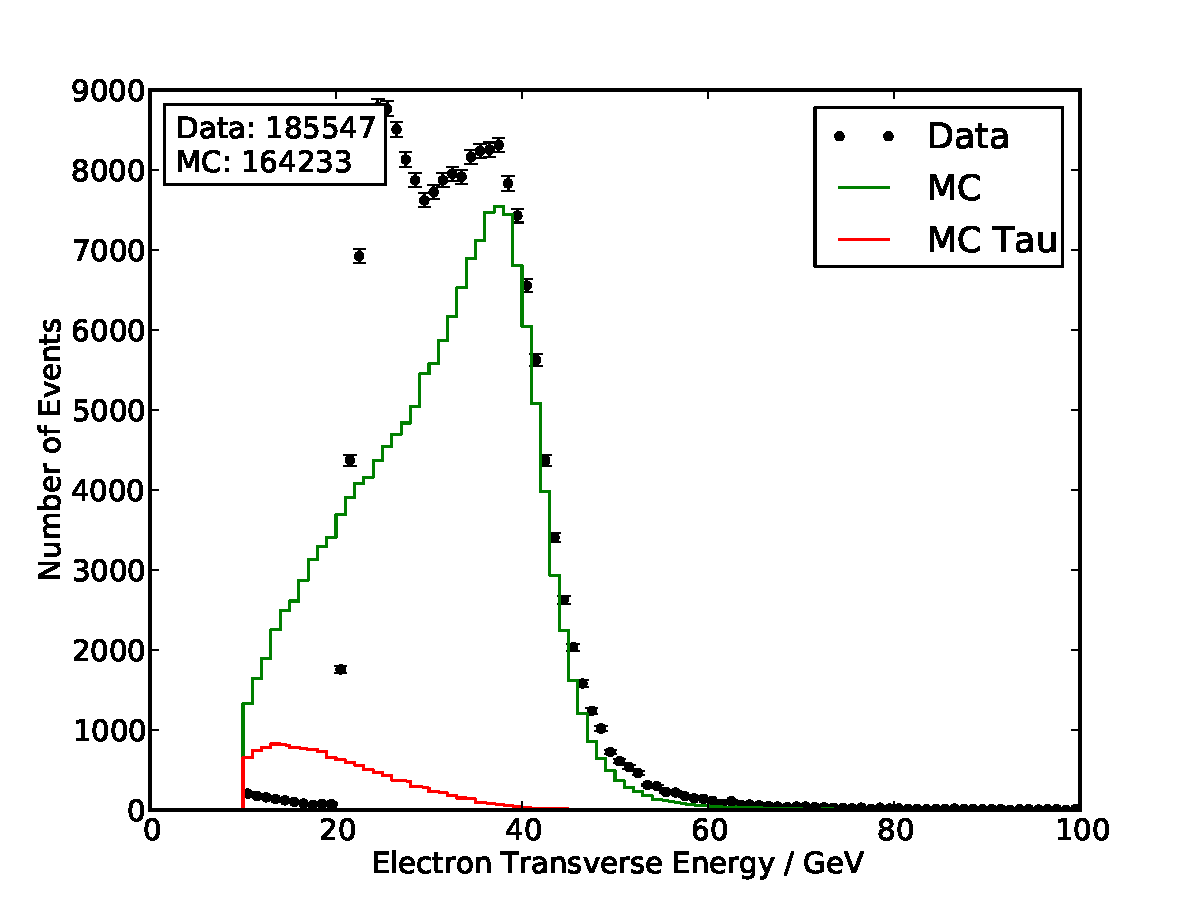
\includegraphics{./nocuts/E_T_el}
		\caption{Distribution of Transverse Electron Energy measured in the Central Calorimeter.}
	\end{subfigure}
	\begin{subfigure}{0.45\textwidth}
		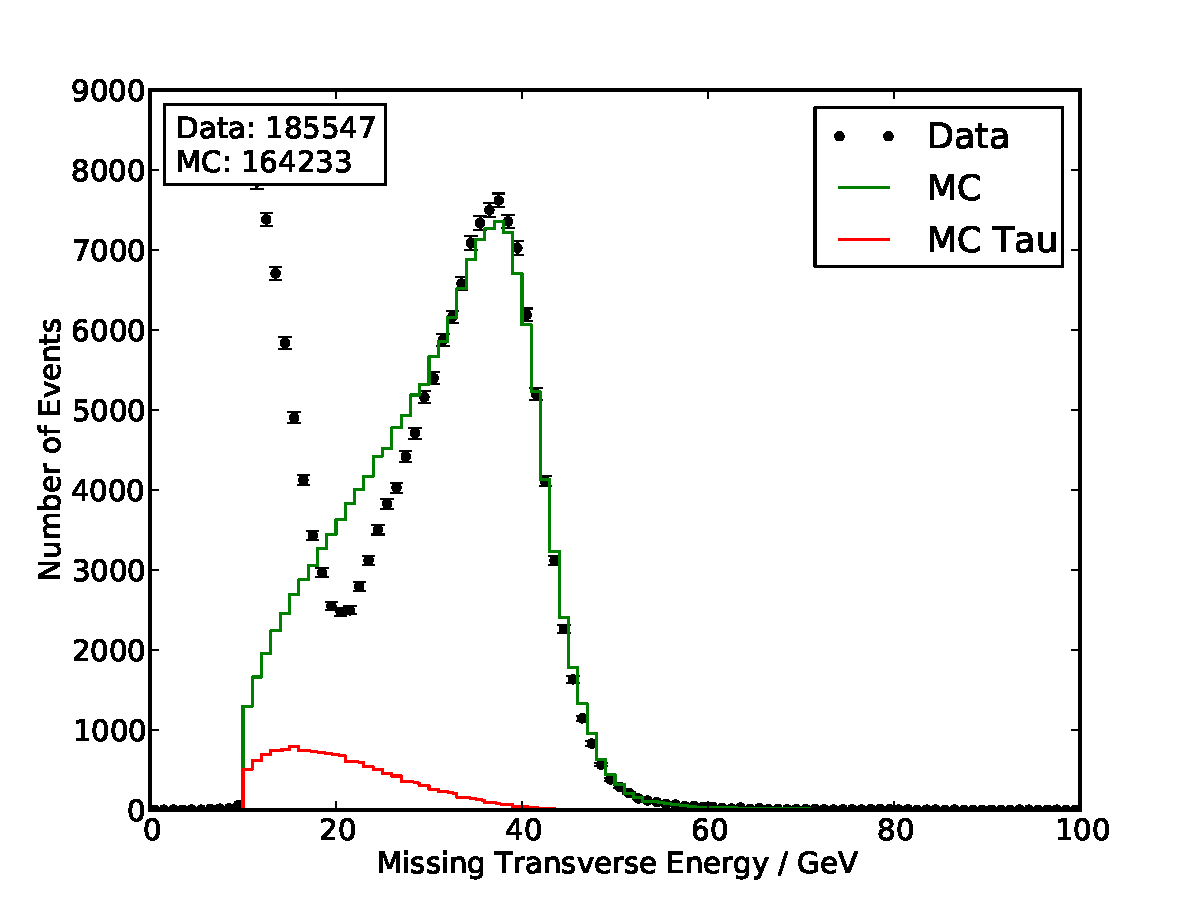
\includegraphics{./nocuts/E_T_miss}
		\caption{Distribution of Missing Transverse Energy, calculated using the constraint of momentum conservation in the transveral plane.}
	\end{subfigure}
	\label{no_cuts_Ets}
\end{figure}

\begin{figure}%
	\centering
	\begin{subfigure}{0.45\textwidth}
		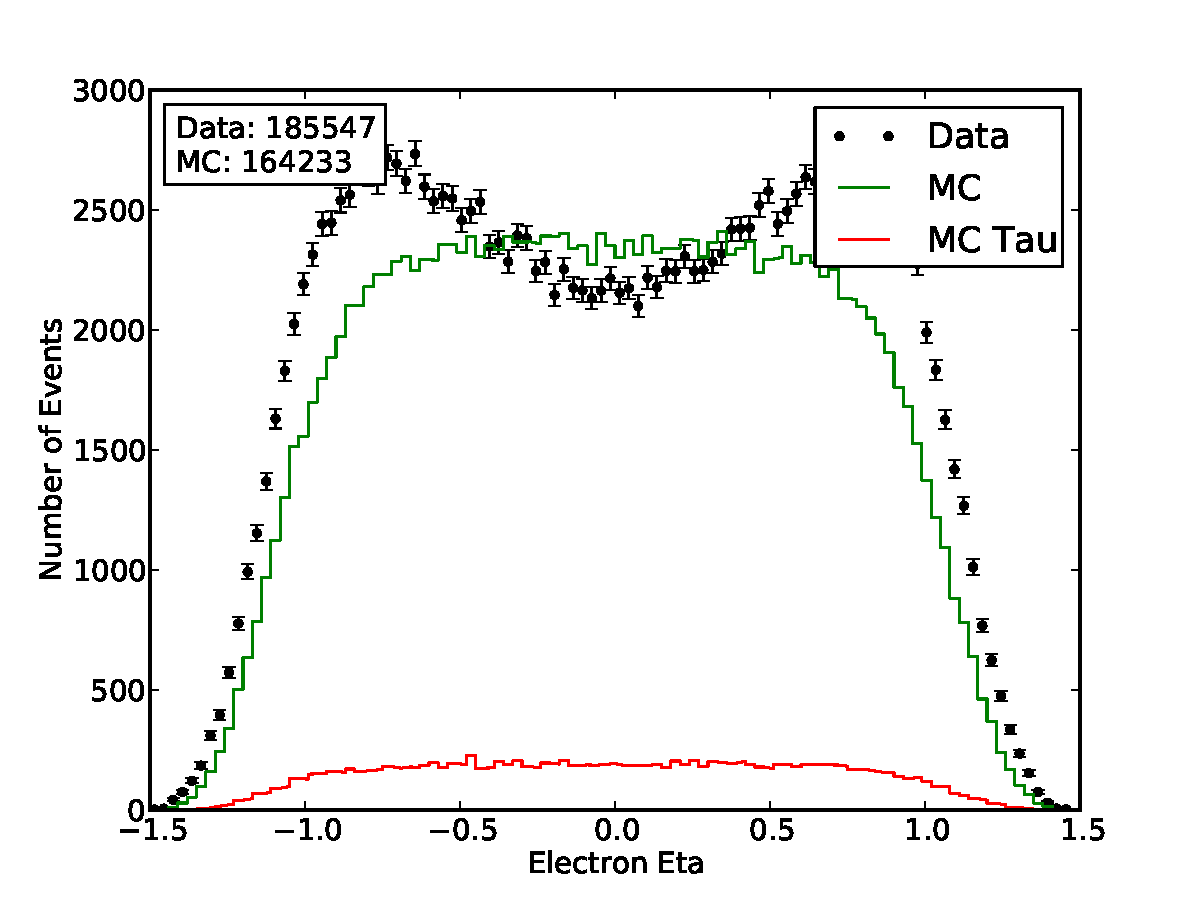
\includegraphics{./nocuts/eta_el}
		\caption{Distribution of the Pseudorapidity of the Electron.}
	\end{subfigure}
	\begin{subfigure}{0.45\textwidth}
		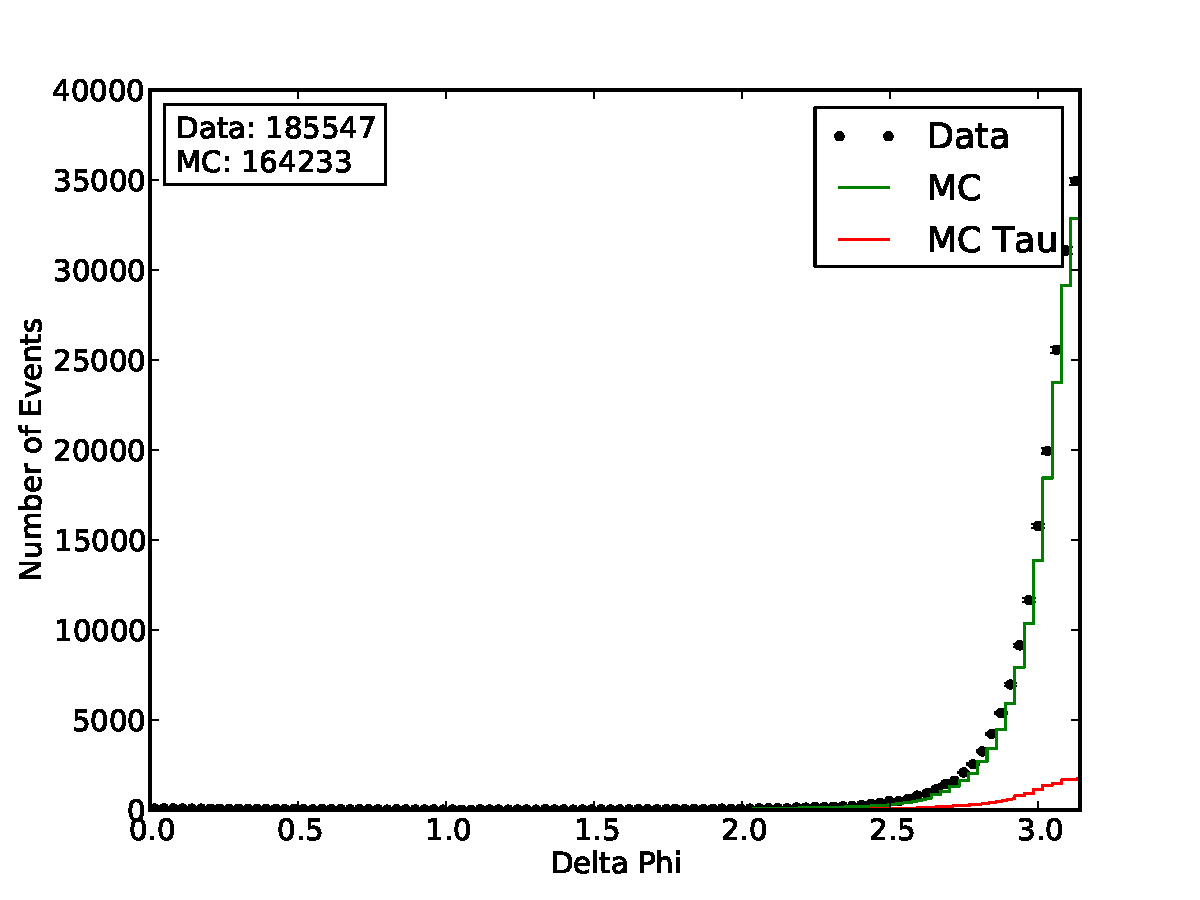
\includegraphics{./nocuts/delta_phi}
		\caption{Distribution of the Difference in Polar Angle $\Phi$ between the directions of MET and the electron.}
	\end{subfigure}
	\label{no_cuts_etaphi}
\end{figure}

\begin{figure}%
	\centering
	\begin{subfigure}{0.45\textwidth}
		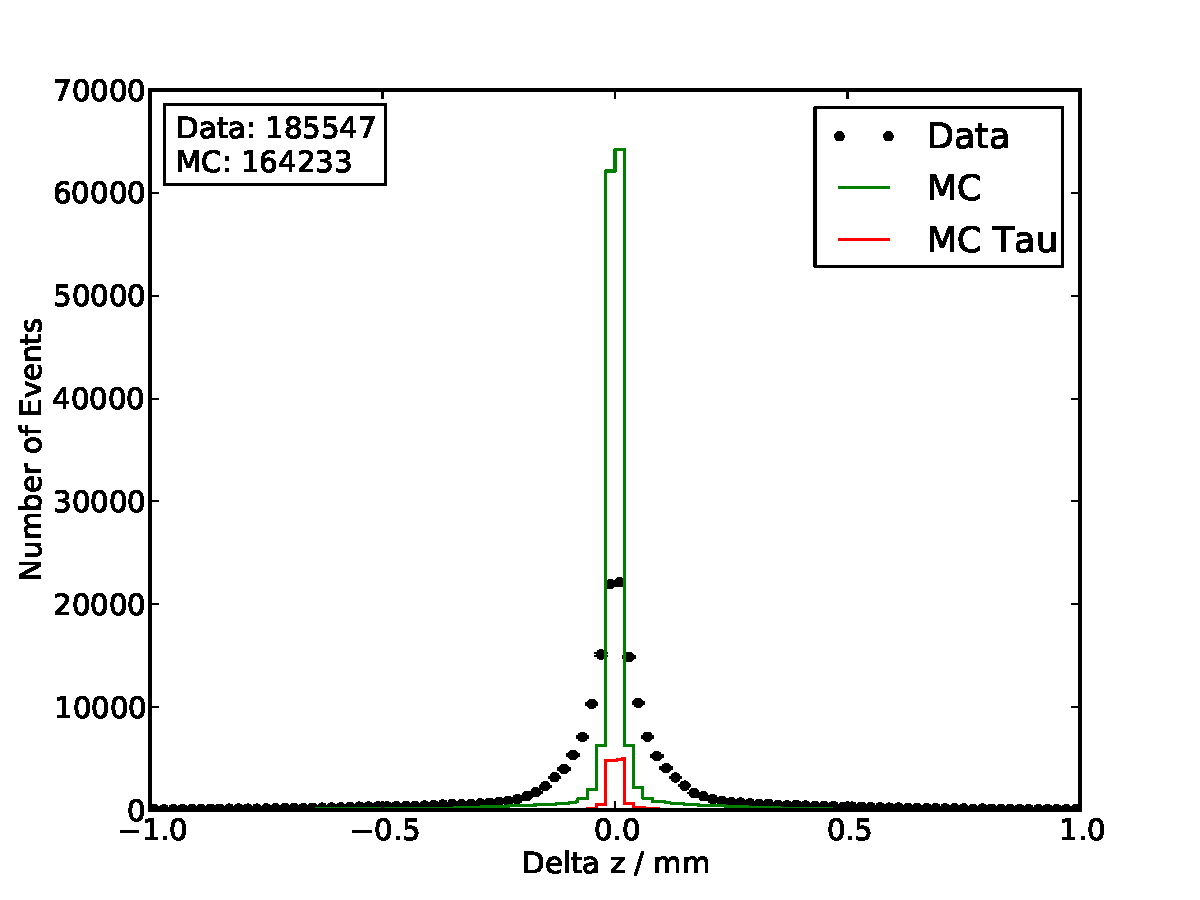
\includegraphics{./nocuts/delta_z}
		\caption{Distribution of the distance of the intersection point between MET and electron track to the collision point.}
	\end{subfigure}
	\begin{subfigure}{0.45\textwidth}
		\includegraphics{Example}
		\caption{Distribution of the Isolation variable describing the tidiness in the vicinity of the electron\'s impact in the EM calorimeter}
	\end{subfigure}
	\label{no_cuts_dziso}
\end{figure}


\cleardoublepage

\bibliographystyle{utphys}
\bibliography{T17_bib}{}

\end{document}
